\chapter{Low-Level and Mid-Level feature analysis for Networked Music Performance}
\label{Chap:NMP}

%\section{Introduction} \label{sec:NMP:introduction}

In the latest decade, the speed and diffusion of the Internet connections have experienced a tremendous improvement. This scenario has made possible the development of novel applications and paradigms such as the services to stream music directly from the Internet or softwares to listen to music with the tempo that matches the user's running pace.

Among the many applications that are crucially dependent on the fast Internet connections, the Networked Music Performance (NMP) promises to revolutionize interactive music fruition (e.g. remote rehearsals, music teaching) by allowing remote players to interact with each other in a musical performance from remote physical locations through an Internet connection over a telecommunication network. Networked Music Performance is a mediated interactional modality with a tremendous potential impact on professional and amateur musicians, as it enables real-time interaction from remote locations.

One  of the known limiting factors of distributed networked performances is the impact of the unavoidable packet delay and jitter introduced by IP networks, which make it difficult to keep a stable tempo during the performance. Computer-based systems enabling music performance have been investigated starting from the \lq 70s \cite{barbosa2003displaced} and recently different network architectures have been proposed as enabling design paradigms for NMP systems, ranging from client-server \cite{saputra2012design,gu2005network} and master-slave \cite{renwick2012sourcenode} to decentralized peer-to-peer infrastructures \cite{stais2013networked,chafe2011living}. 

%The delay tolerance is typically estimated to be 20-30 ms \cite{carot2009fundamentals} (corresponding to the time that the sound field takes to cover a distance of 8-9 m), which has been shown to correspond to the maximum physical separation beyond which keeping a common tempo for rhythmic music interaction without conductor becomes difficult. However, the sensitivity to delay and the quality of the musical experience in the context of NMP is influenced by several additional factors \cite{Bouillot2007}. In \cite{barbosa2011influence}, the authors investigate the correlation between perceptual attack times of the instrument (i.e., the time that the instrument takes to reach its maximum loudness) and the sensitivity to network delay, concluding that instruments with a slow attack (e.g. strings) usually tolerate higher latency. In \cite{Chew2004}, the authors investigate the correlation between accepted network latency and the genres of pattern-based music. 

The above mentioned studies employ a qualitative analysis of the additional factors to investigate their correlation with the sensitivity to delay and the overall quality of the music performance. In \cite{barbosa2011influence}, two classes of instruments are defined, with slow or fast attack times, and it is found that the presence of the former class of instruments helps the musicians to be less sensible to the latency. In \cite{Chew2004} some broad class of genres are defined to investigate their correlation with the tolerance to the network latency. However, a quantitative analysis can be more useful to understand the issues raised by NMP and to relax the latency constraints for the design of the network architecture.

We aim at conducting a quantitative study about the effects of some acoustic properties on the musicians' tolerance to the delay and on the quality of music performance. We perform the quantitative study by taking advantage of the dimensional feature-based representation of music analysis \cite{Kim2005,Zanoni2012}. More specifically, we investigate which factors affect the subjective and objective quality of a NMP and, therefore, which network constraint must be satisfied depending on the different properties of the music.

We model the problem of the NMP as a linking function from the music performance to its objective and subjective quality of the performance itself. We are interested in the objective qualities of the music, therefore the signal domain is formalized by means of a set of low-level and mid-level features. The semantic codomain is represented by means of some quality metrics, for which we extract the trend of the tempo kept during the performance and we collect annotations from the musicians about the perceptual quality of the musical interaction. We investigate the quantitative correlation between the signal domain and the semantic codomain by modeling the linking function as a manual data analysis.

In the following we provide an overview of the state of the art and theoretical background on NMP (Section \ref{sec:NMP:background}). In order to conduct this analysis, we implemented a testbed for psycho-acoustic analysis emulating the behavior of a real IP network in terms of variable transmission delay and jitter, and we recorded a set of NMPs with different musicians, instruments, songs and tempo within the song. We present the details on the setup of the testbed in Section \ref{sec:NMP:testbed}. The obtained recording are processed in order to extract the features for the signal domain and the quality metric for the semantic codomain. We describe the extraction techniques in Section 
\ref{sec:NMP:domain}. Finally, in Section \ref{sec:NMP:results} we present the results of the manual analysis of the collected data and we draw some final considerations in Section \ref{sec:NMP:conclusions}.

In our study we conducted a set of experiments with both male and female musicians. In the following discussion, therefore, we use the \textit{singular they} with the gender-neutral meaning. 

%such as the rhythmic complexity of the performed piece, the timbral characteristics of the instruments and the type of musical part that is being performed (e.g. melody, chord comping, sustained harmony) has not yet been proposed in the literature. 


\section{Background}\label{sec:NMP:background}
In order to reproduce realistic environmental conditions for NMP, several technical, psycho-cognitive and musicological issues must be addressed. In particular, at network level, very strict requirements in terms of latency and jitter must be satisfied to keep the one-way end-to-end transmission delay below a few tens of milliseconds. 

The overall delay experienced by the players includes multiple contributions due to different stages of the audio signal transmission: the first is the processing delay introduced by the audio acquisition, processing, and packetization; the second is the pure propagation delay over the physical transmission medium; the third is the data processing delay introduced by the intermediate network nodes traversed by the audio data along their path from source to destination, the fourth is the playout buffering which might be required to compensate the effects of jitter in order to provide sufficiently low packet losses to ensure a target audio quality level.

Some preliminary studies on the delay tolerance for live musical interactions have already appeared: in \cite{gurevich2004simulation,chafe2010effect,chafe2004effect,chafe2004network} the authors evaluated the trend of tempo variations (measured in Beats Per Minute - BPM) while performing predefined rhythmic patterns through hand clapping, in different latency conditions. A similar analysis was integrated with an evaluation of the musicians' subjective rating of the performance quality in \cite{carot2009towards}. In \cite{barbosa2011influence}, the authors show that the human auditory system focuses on onsets produced by instruments with a short or almost impulsive attack time, whereas it tends to perceive less immediately those onsets associated to instruments with a slow attack. The impact of delay on the synchronism of the performance is therefore expected to be more clearly perceivable when using musical instruments with a fast attack, rather than when using instruments with a slower attack time. This means that the choice of musical instrument matters in presence of network delay. In practice, however, musicians tend to adjust their playing technique according to the specific attack time of the instrument played. For example, organ players are used to naturally compensating the delay elapsed between the pressure of the keyboard keys and the sound emission from the pipes, as well as the time that the sound takes to travel back from the pipes to the musician. To a smaller extent this is also true for piano players. In this case the delay between pressing a key and detecting the corresponding note onset varies between $30$ and $100$ ms, depending on sound loudness and musical articulation (e.g. \textit{legato, staccato}) \cite{askenfelt}. For some categories of instruments, it has been shown that the expressive intention and direction of the musician (i.e., subjective artistic and interpretation choices, which are in turn affected by a particular emotional state during the performance) can have a significant impact on sonological parameters such as attack, sustain and decay time \cite{clarinet}. In our study we do not evaluate the impact of the instrument attack time on the performance interplay, and consider this attack time simply as part of the overall delay perceived by the musician. 

One specific aspect that needs to be addressed is the role played by a musical instrument in a performance. In western music, some instruments have a more pronounced ``leading'' role than others. In \cite{Carot07networkmusic} the authors define two main musical roles, the \textit{solo} and the \textit{rhythmic} parts, and they identify some approaches of musical interaction that depend on the network delay that is set. The best situation is called \textit{Realistic Interaction Approach} (RIA), when the network delay is lower than 25 ms, both roles can play with total interaction as if they were playing in the same physical place. Beyond the 25 ms threshold, the performance usually shifts to a \textit{Master-Slave Approach} (MSA), where the rhythmic part leads the interaction with the solo part, as the Master of the performance, and the the solo part follows the provided tempo, acting as the Slave. The rhythmic players are therefore expected to keep a steady tempo even when the other musicians are playing off-tempo. From the solo perspective, the synchronization is good, while the interaction is more difficult. When the delay approaches the 50 ms value, \cite{Carot07networkmusic} suggests a behavior named \textit{Laid Back Approach} (LBA), whereby the solo plays slightly behind the groove led by the rhythmic part. This approach is a common solo style in jazz music and produces an acceptable interaction for the musicians even if for high delay. An alternative MSA approach is the \textit{Delayed Feedback Approach} (DFA), where the rhythmic part holds its leading role, while receiving their own sound feedback with a slight delay. If the delay of the feedback is similar to the network delay, the rhythmic musician will listen to their feedback in sync with the solo part. In DFA, the solo musician perceives a synchronization quality similar to the MSA, while it is more challenging for the rhythmic musician to handle the delayed feedback. 

In our study we extend the set of roles to four, where we split the rhythmic parts into chord comping and drums, and we include the sustained harmony. For this reason, we do not use the taxonomy of approaches defined by \cite{Carot07networkmusic}.


\section{Testbed setup}\label{sec:NMP:testbed}
\begin{figure}[!tb]
  \centering
  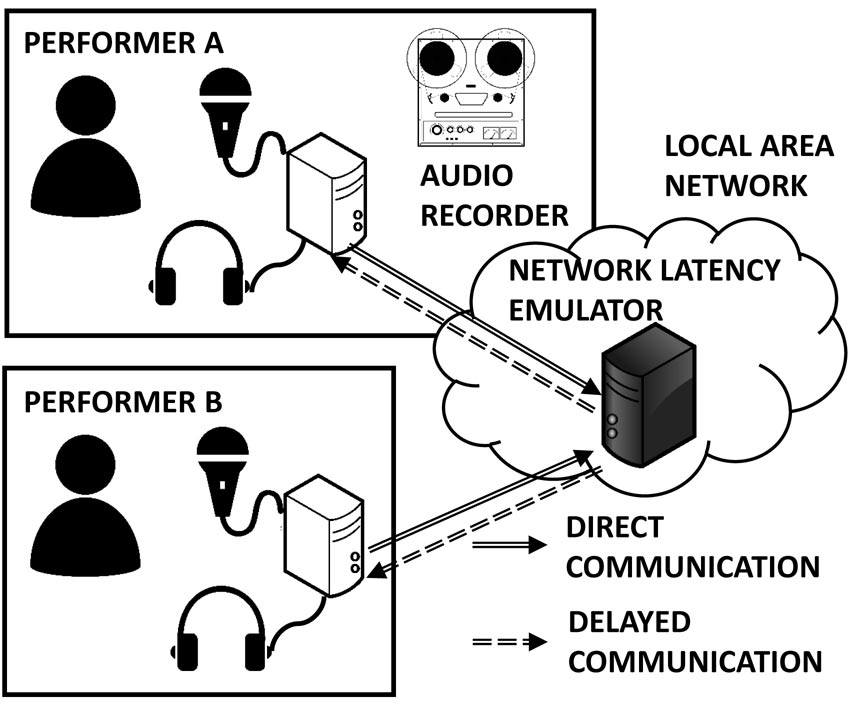
\includegraphics[width=.95\textwidth]{img/NMP/setup}
  \caption{Testbed setup}
 \label{fig:NMP:testbed}
\end{figure}
In order to analyze the correlation of the music played with the tolerance to delay, we implemented a testbed setup to emulate the NMP scenario. Our experiments involved pairs of musicians playing in two phono-insulated near-anechoic rooms (sound rooms), to avoid any audio feedback or visual contact, as depicted in Figure \ref{fig:NMP:testbed}. Visual contact was provided not even by means of video streaming because video processing time is larger than audio processing time and would have increased the minimum achievable end-to-end delay. The musicians were also forbidden to verbally communicate to their counterpart during the performance. Each room was equipped with a desktop PC running the Soundjack software, which is a peer-to-peer publicly available software \cite{carot2008distributed} that also implements a direct real-time evaluation of the experienced one-way end-to-end latency (thus including processing, buffering and playout delays).  Each PC was connected to an external sound card via high-speed connection (FireWire and AES/EBU) operating at a sampling rate of 48 kHz. The sound card was connected to high-quality headphones and microphones. An additional PC (with two network interfaces) running the WANem network emulator \cite{wanem} was placed in between. 
The WANem emulator allows the users to manually select the delay and jitter of the emulated network, in order to replicate the NMP real-world scenario. The network interfaces of the three PCs were connected to each other through a Fast Ethernet switch. The PCs of the sound rooms were configured to communicate exclusively through the interfaces of the WANem emulator, thus preventing any direct communication between them. 

Each musician was able to hear their own instrument as well as the instrument of the other player through headphones. The choice of the headphones was made in order to minimize the possible delay and to avoid loop-feedback effects. The two audio signals were transmitted through the Local Area Network of the building. During the experiments, all the involved LAN segments were free of other traffic. The audio tracks were recorded as follows: the audio data generated by \textit{performer A} were recorded directly after the electric transduction of the microphone, whereas the audio data generated by \textit{performer B} were recorded from the SoundJack feedback after propagation of the audio stream through the network, i.e. as heard through \textit{performer A}'s headsets.

%\subsection{Scores and Network Parameters}
We considered three different music pieces: \textit{Yellow Submarine} (by The Beatles) at different values of BPM (88,110,130), \textit{Bolero} (by Maurice Ravel), and \textit{Master Blaster} (by Stevie Wonder), arranged for four different parts: main melody (M), chord comping (CC), sustained harmony (SH), and drums (D).  Scores were released to the musicians in advance.

\begin{table}[tb]
  \caption{Combination of parts played in each experiment session. M: main melody; CC: chord comping; SH: sustained harmony; D: drums}
  \centering %\small
  \label{tab:NMP:sessions}
  \bgroup
  \def\arraystretch{1.5}
 \begin{tabular}{||c|c|c|c|c||}
 \hline
 \hline
  Id & Instrument A& Part A & Instrument B & Part B \\
 \hline
 \hline
  1 & Acoustic Guitar & M & Classic Guitar & CC\\
  2 & Electric Piano & M & Drums & D\\
  3 & Keyboard (strings)  & SH & Drums & D\\
  4 & Keyboard (strings)  & SH & Electric Guitar & CC\\
  5 & Clarinet & M & Clarinet & M\\
  6 & Eletric Guitar  & CC & Drums & D\\
  7 & Keyboard (strings)  & SH & Clarinet & M\\
 \hline
 \hline
   \end{tabular}
   \egroup
\end{table}

Our experiments involved 8 musicians with at least 8 years of musical experience, all with semi-professional or professional training level, and 7 instruments, i.e.:
Acoustic, Classic and Electric Guitar, Clarinet, Drums, Electric Piano and Keyboards with strings samples. Each musician played at least one of the instruments. The musicians were grouped in 7 pairs according to the combinations listed in Table \ref{tab:NMP:sessions}. Note that some musicians performed in more than one pair (e.g., one clarinetist performed twice, i.e. in pairs 5 and 7, whereas the pianist played electric piano and keyboard in pairs 2, 3, 4 and 7). For a given pair, each musician performed only one of the four parts for each of the three considered musical pieces, as detailed in Table \ref{tab:NMP:sessions}. Musicians in pairs 5 and 6 had regularly performed together in the last years, where the remaining pairs had never played together before. However, in order to avoid biases due to prior common performances, all the pairs were allowed to practice together in the testbed environment until they felt sufficiently confident. Before participating to our experiments, none of the players had ever experienced networked music interactions.

\begin{table}[tb]
  \caption{Tested network parameters and tempo settings}
  \centering %\small
  \label{tab:NMP:param}  
  \bgroup
  \def\arraystretch{1.5}
  \begin{tabular}{||c|c|c|c||}
\hline
\hline
 Piece & $\delta$ [BPM]& $\mu$ [ms]& $\sigma$ [ms]\\
\hline
\hline
 Yellow Submarine & 88,110,132 & 20,30,40,50,60 & 1 \\
 Bolero & 68  & 20,30,40,50,60 & 1 \\
 Master Blaster & 132  & 20,30,40,50,60 & 1 \\
\hline
\hline
  \end{tabular}
  \egroup
\end{table}

The recording procedure was repeated several times for each piece. As reported in Table \ref{tab:NMP:param}, each recording was characterized by different tempo and network settings in terms of reference BPM ($\delta$), network latency and jitter. The two latter parameters were set by assigning each IP packet a random delay $T_{net}$, statistically characterized by independent identically distributed Gaussian random variables with mean $\mu$ and standard deviation $\sigma$. The payload of each packet contained $128$ 16-bit-long audio samples, corresponding to a duration of $2.67$ ms. For the considered values of $\mu$ and $\sigma$, we set the receiver buffer size to 4 packets (i.e. $512$ audio samples) and measured the number of buffer overruns/underruns during each recording. The overall probability of overrun/underrun events turned out to be smaller than $1\%$. This value is representative of realistic traffic conditions of a telecommunication network. Note that overruns/underruns generate glitches (e.i, distortions in the reproduction of the received audio signal) which affect the overall audio quality perceived by the musicians. 
 

Note also that, as $T_{net}$ accounts only for the emulated network delay, the additional latency $T_{proc}$ introduced by the audio acquisition and the audio rendering processes must be taken into account in the computation of the one-way overall delay time $T_{tot}=T_{net}+ T_{proc}$.
More specifically, the processing time $T_{proc}$ includes: in-air sound propagation from instrument to microphone; transduction from the acoustic wave to electric signal in the microphone; signal transmission through the microphone's wire; analog to digital conversion of the sender's sound card, internal data buffering of the sound card; processing time of the sender's PC to packetize the audio data prior to transmission; processing time of the receiver's PC to depacketize the received audio data; queuing time of the audio data in the application buffer at the receiver side; digital to analog conversion of the receiver's sound card; transmission of the signal through the headphone's electric wire; transduction from electric signal to acoustic wave in the headphones.
We experimentally evaluated $T_{proc}$ by measuring the end-to-end delay $T_{tot}$ when setting $\mu=0$ and $\sigma=0$, i.e., $T_{net}=0$. The measured time was $T_{proc}=15$ ms, which is larger than the one reported in \cite{carot2007networked}. This is mainly due to the use of generic sound card drivers, which increased the processing time of SoundJack.

During each recording session, the order of the proposed network configurations was randomly chosen and was kept undisclosed to the testers, in order to avoid biasing or conditioning. Two measures of metronome beats at the reference BPM were played before the beginning of each performance. At the end of each performance, the testers were asked to express a rating on the quality of their interactive performance. The details on such quality are provided in the next Section.

\section{Collection of the signal domain and the semantic codomain}\label{sec:NMP:domain}
We formalize the signal domain by extracting rhythmic and timbral features from the recordings of the performance and from the score of the parts. The semantic codomain is evaluated by means of subjective quality metrics, asked to the musicians after each performance, and of objective quality, through a processing technique from the recordings.


\subsection{The signal domain}\label{sec:NMP:domain}

\begin{table}[tb]
  \caption{Timbral characterization for each instrument}
  \centering %\small
  \label{tab:NMP:instruments}
  \bgroup
  \def\arraystretch{1.5}
\begin{tabular}{||c|c|c|c|c|c|c||}
 \hline
 \hline
 Instrument  & $SC$ & $SSp$ & $SSk$ & $SK$ & $SF$ & $SE$ \\
 \hline
 \hline
Ac. Guitar &   2047 & 4109 & 2.76 & 10.25 & 0.19 & 0.76 \\
Clarinet & 1686 & 2272 & 4.85 & 31.81 & 0.07 & 0.731 \\
Cl. Guitar &   3263 & 4680 & 1.57 & 4.43 & 0.22 & 0.841 \\
Drums & 7903 & 7289 & 0.35 & 1.57 & 0.61 & 0.936 \\
El. Guitar & 1848 & 2522 & 3.70 & 23.46 & 0.09 & 0.818 \\
El. Piano & 2101 & 4251 & 3.16 & 12.26 & 0.16 & 0.734 \\
Keyboard & 1655 & 3065 & 4.39 & 23.77 & 0.1 & 0.733 \\
 \hline
 \hline
   \end{tabular}
   \egroup
\end{table}

As far as the timbral features are regarded, we consider the timbre as a property of the instrument and we do not track their evolution during the performances. For each instrument, we compose an audio file with a representative selection of recordings of its timbre. For example, the timbral characterization of the drums included the recording of each percussive instrument from the drum set, whereas the characterization of guitar included different kinds of playing techniques, like chords played as arpeggio and plucked strings. From the representative audio files we then extract the following features: Spectral Centroid ($SC$), Spectral Spreadness ($SSp$), Spectral Skewness ($SSk$), Spectral Kurtosis ($SK$), Spectral Flatness ($SF$) and Spectral Entropy ($SE$). The definition and interpretation of such features was provided in Section \ref{sec:LLFs:LLFs}. It is worth remembering that the Spectral Centroid provides an indicator of the brightness of the timbre, while Spectral Entropy and Flatness can be interpreted as an estimate of the noisiness. 

The features are extracted by means of the MIRToolbox \cite{Lartillot2007} and their average values computed over each audio file are reported in Table \ref{tab:NMP:instruments}. We can notice that the Drums exhibit the highest values of Flatness and Entropy, hence noisiness, and a rather high Spectral Centroid. On the other side, the Clarinet presents the lowest value of noisiness and a low Spectral Centroid, given by its warm deep timbre. Among the guitars, we do not use distortion effect for the Electric Guitar, hence its timbre is rather clean and has a lower Spectral Flatness than the Acoustic Guitar, while showing a higher Entropy.

\begin{table}[tb]
  \caption{Rythmic characterization of the musical pieces performed during the tests}
  \centering %\small
  \label{tab:NMP:pieces}  
  \bgroup
  \def\arraystretch{1.5}
 \begin{tabular}{||c|c|p{1.4cm}|p{1.4cm}|p{1.8cm}|p{1.8cm}|p{1.8cm}||}
 \hline
 \hline
Part &	Feature & Bolero & Master Blaster & Yellow Submarine (88 BPM) & Yellow Submarine (110 BPM) & Yellow Submarine (130 BPM)\\
 \hline
 \hline
 \multirow{2}{*}{M}& ED & 2.1407 & 2.1667 & 1.5253 & 1.9067 & 2.2880 \\
 				   & RC & 5.5337 & 5.5627 & 5.4160 & 5.7094 & 6.0567 \\
\hline
\multirow{2}{*}{CC}& ED & 1.3222 & 2.6542 & 1.8333 & 2.2917 & 2.7500 \\
				  & RC & 3.4516 & 6.8903 & 5.3064 & 5.6455 & 5.9592\\
\hline
\multirow{2}{*}{SH}& ED & 0.3778 & 0.5778 & 0.8213 & 1.0267 & 1.2320 \\
 				  & RC & 2.9364 & 5.3444 & 3.8062 & 4.0208 & 4.2237\\
\hline
\multirow{2}{*}{D}& ED & 2.0148 & 4.3514 & 1.5253 & 1.9067 & 2.2880 \\
			   & RC & 6.0285 & 5.7255 & 4.5228 & 4.7548 &  4.9767 \\
 \hline
 \hline
   \end{tabular}
   \egroup
\end{table}

As far as the rhytmic features are regarded, we extract some of the MLFs described in Section \ref{sec:LLFs:MLFs}, i.e., the Tempo, the Rhythmic Complexity and the Event Onset. As mentioned, the tempo was fixed and provided to the musician, and a particular song, \textit{Yellow Submarine}, was executed at different tempi. We manually compute the Event Density \cite{Lartillot2007} from the sheet music of the parts and we extract the Rhytmic Complexity \cite{povel} using the MIDI Toolbox \cite{Eerola2004}. With reference to the Equation \ref{eq:RC}, we use the weights $w_1= 0.7$, $w_2=0.2,$  $w_3=0.5$, $w_4=0.5$, i.e., the Entropy of the distribution of the notes has the greatest relevance, then the standard deviation of the distribution of the notes and the the synchrony of phenomenal accent in the score are equally weighted and finally, the Event Density receives a low weight. 

The rhythmic features for each part are summerized in Table 
\ref{tab:NMP:pieces}. We can notice that the Sustained Harmony has generally low values of Event Density and Rhytmic Complexity, since it usually involves one onset every measure. On the other side, the Chord Comping of \textit{Master Blaster} and the drums in \textit{Bolero} are rhythmically challenging, due to the variation between even and odd patterns. Moreover, since the Event Density depends on the tempo and Rhytmic Complexity depends on Event Density, we can notice that increasing the BPM of \textit{Yellow Submarine} produces an increase of both features.




%in this study we provide an evaluation of the impact of network conditions on the quality of the musical experience, according to the type of the instruments and to some characteristics of the performance. As far as the type of instrument is concerned we adopt a timbral feature-based representation, whereas we exploit musical part, Event Density \cite{Lartillot2007} and Rhythmic Complexity \cite{povel} of the performed pieces to characterize the performance. 

\subsection{The semantic codomain}\label{sec:NMP:codomain}
In the NMP scenario, the semantic codomain is represented by the quality of the performance over the network. We define three metrics of quality, two subjective metrics annotated by the musicians  and one objective metric that is the trend of the tempo over the performance.

At the end of each of the recordings described in the previous Section, we asked to the musicians to rate the quality of the performance. The musicians provided two annotations: one about the quality of the interaction and one about the perception of the delay. The former is defined as the perceived quality $Q_{perc}$, and is annotated within a five-valued range, from $Q_{perc}=1$, meaning the performance was very poor, to $Q_{perc}=5$, i.e., very good. The metric $Q_{perc}$ is not related to the audio quality experienced by the musicians, but only to the evaluation of the overall satisfaction of their experience and interaction with the counterpart. The latter is defined as the perceived network delay, $D_{perc}$, and it ranges between $1$, i.e., the delay is intolerable, and $4$, i.e., the delay was not perceivable. In case the players spontaneously aborted their performance within the first $50$ seconds, $D_{perc}$ was set to $1$ and $Q_{perc}$ was set to $0$ by default. 

After the recording sessions, we extract the objective quality metric as the trend of the tempo during the performances, i.e., the tendency to slow down or accelerate in the initial part of the performance. For the first $50$ seconds we compute a linear regression of the BPM over the sparse BPM measurements. In order to do so, we first manually annotate the beats of the performance, as it is indicated in the music score. We estimate the beats occurring in the silences as equally distant from the surrounding beats. We are able to compute the instantaneous BPM from the time difference between two consecutive beats. We compute the BPM trend by smoothing the sequence of instantaneous BPM. The audio tracks are divided in $N=20$ time windows, each lasting $5$~s, with a 50\% overlap ($2.5$~s). For each time window, we compute the average BPM as $b(t_n)$ with $t_n=n*2.5$s and $n=1,...,N$. We estimate the tendency of the performance to accelerate or decelerate by considering the slope of the linear approximation of the BPM trend. We estimate the intercept $\beta$ and the slope $\kappa$ with linear interpolation, 
\begin{equation}
\argmin{\kappa, \beta} \frac{1}{N} \sum_{n=1}^{N} \left(b(t_n)-(\kappa t_n + \beta)\right)^2.
\end{equation}
In our experiments, the average Mean Square Error of the linear approximation is about $1.75$\%, i.e., it is accurate to approximate the BPM trend as a first order polynomial.

We consider the slope $\kappa$ as the objective metric for the evaluation of the performance quality: $\kappa=0$ means steady tempo; $\kappa>0$ means that the musician is accelerating; $\kappa<0$ means that the musician is slowing down and thus is unable to keep up with the tempo. 

\section{Numerical results}\label{sec:NMP:results}
In this Section, we build the linking function by means of a manual data analysis. We first provide some general and qualitative considerations on the BPM trend of the performance, and then we discuss the quantitative analysis of the NMP.

\subsection{Qualitative evaluation}
\begin{wrapfigure}{r}{0.3\textwidth}
  \begin{center}
     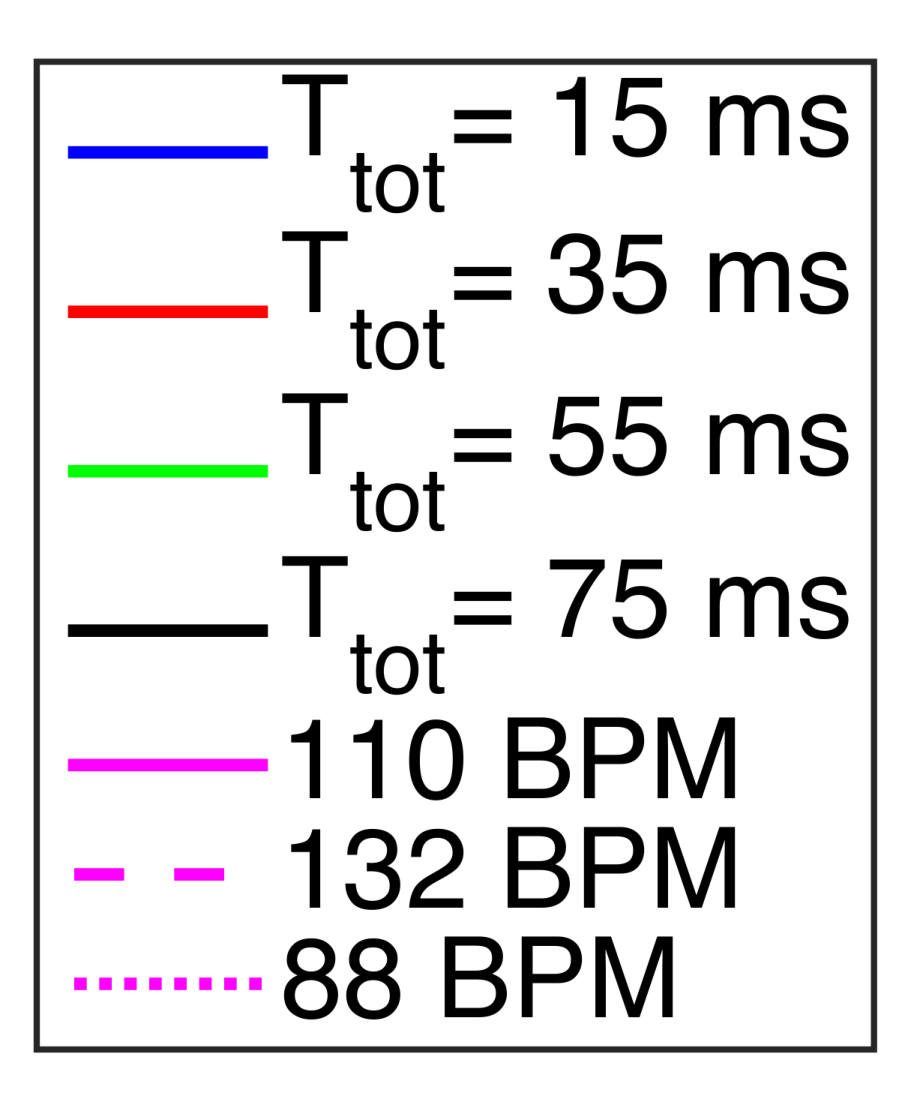
\includegraphics[width=0.2\textwidth]{img/NMP/legend_smaller}
  \end{center}
  \caption{Legend for Figures \ref{fig:NMP:melody} and \ref{fig:NMP:drums} }
 \label{fig:NMP:legend} 
\end{wrapfigure}

We begin with some qualitative comments on the trend of the BPM curve $b(t_n)$ extracted from %the first $50$ s of
the execution of \textit{ Yellow Submarine} for different combinations of instruments and parts, various values of $T_{tot}$ in the range between $15$ and $75$ ms and three different values of $\delta$ (as reported in Table \ref{tab:NMP:param}). The lower bound of the tested delay values (i.e. $T_{tot}=15$ ms) is obtained by setting $T_{net}=0$ ms, meaning that no network delay is added to the unavoidable processing time $T_{proc}$. For values of $T_{tot}$ above $75$ ms (i.e., when $T_{net}=60$ ms), a considerable amount of executions were aborted by the musicians due to the extreme difficulty in maintaining synchronization. Therefore, we limit our analysis to delay ranges which allowed every pair of musician to perform the piece uninterruptedly for at least one minute.
The results are reported in Figures \ref{fig:NMP:melody} and \ref{fig:NMP:drums}, while the legend is shown in Figure  \ref{fig:NMP:legend}. The different colors identify the amount of total network delay $T_{tot}$ applied, while the style of the lines identifies the nominal BPM. The results show that in all the considered recordings an initial deceleration occurs in the first few seconds, when the players adjust their tempo until they find a balance, allowing them to reach the required degree of synchronization. Such initial deceleration is nearly absent for small network end-to-end delays and reference BPM, but it becomes much more pronounced for large values of $T_{tot}$ and $\delta$. In particular, the scenario with $\delta=132$ BPM and $T_{tot}=75$ ms presents an initial tempo reduction of 12-20 BPM in all the tested combinations of instruments and parts.
In addition, as shown in Figure \ref{fig:NMP:melody}, combining typically non-homorhythmic parts such as Melody (M) and Chord Comping (CC) or M and Sustained Harmony (SH) leads either to a tendency to constantly decelerate (see Figure~\ref{fig:NMP:melody}, left-hand side), which is more pronounced for large $\delta$ , or to a \lq\lq saw tooth'' pattern in which the players periodically try to compensate the tempo reduction (Figure \ref{fig:NMP:melody}, middle). Note that, in the latter case, there is no such pattern in the benchmark scenarios with $T_{tot}=15$ ms. The difference in the behavior of SH and CC when interacting with M is also due to the type of rhythmic interplay that takes place. Chord Comping, in fact, tends to closely follow and match the tempo of the Melody, while Sustained Harmony is a steady accompaniment (``pad") with more relaxed on-time constraints. As M is expected to meander off-tempo, it is harder for SH and M to stay in sync, and adjustments happen in bursts.


\begin{figure}[!tb]
  \centering
  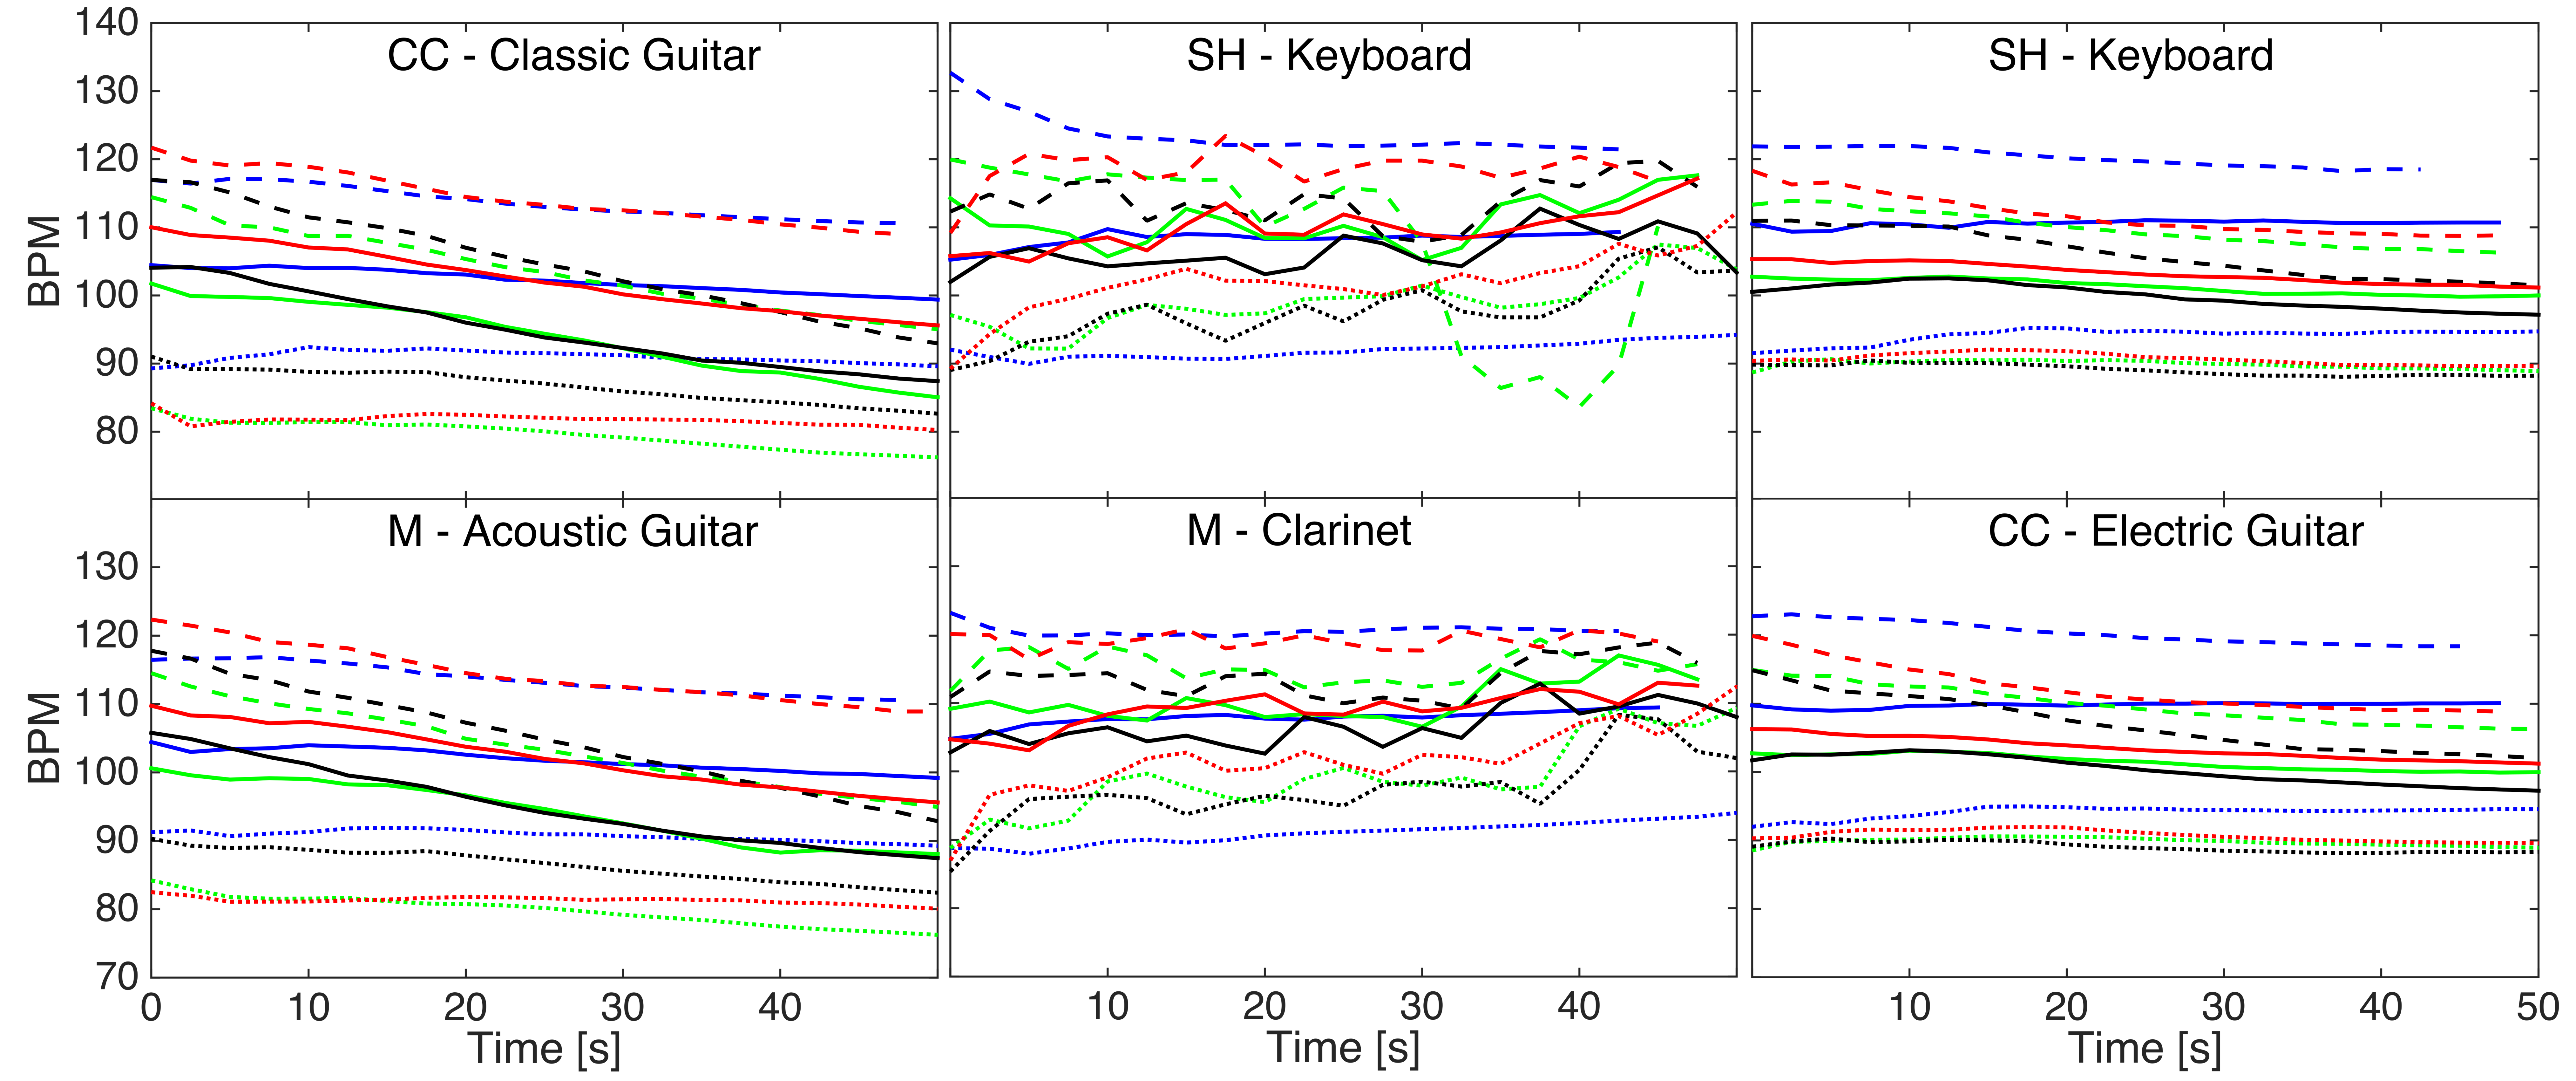
\includegraphics[width=\textwidth]{img/NMP/fig1_wider}
  \caption{BPM trend over time when playing \textit{Yellow Submarine}, for different combinations of parts, instruments,  end-to-end delays $T_{tot}$ (identified by the color) and reference BPM $\delta$, identified by the type of line (solid, dashed, dotted).}
%  (\textit{performer A} on top, \textit{performer B} on bottom), for various values of
   \label{fig:NMP:melody} 
\end{figure}
\begin{figure}[!tb]
  \centering
  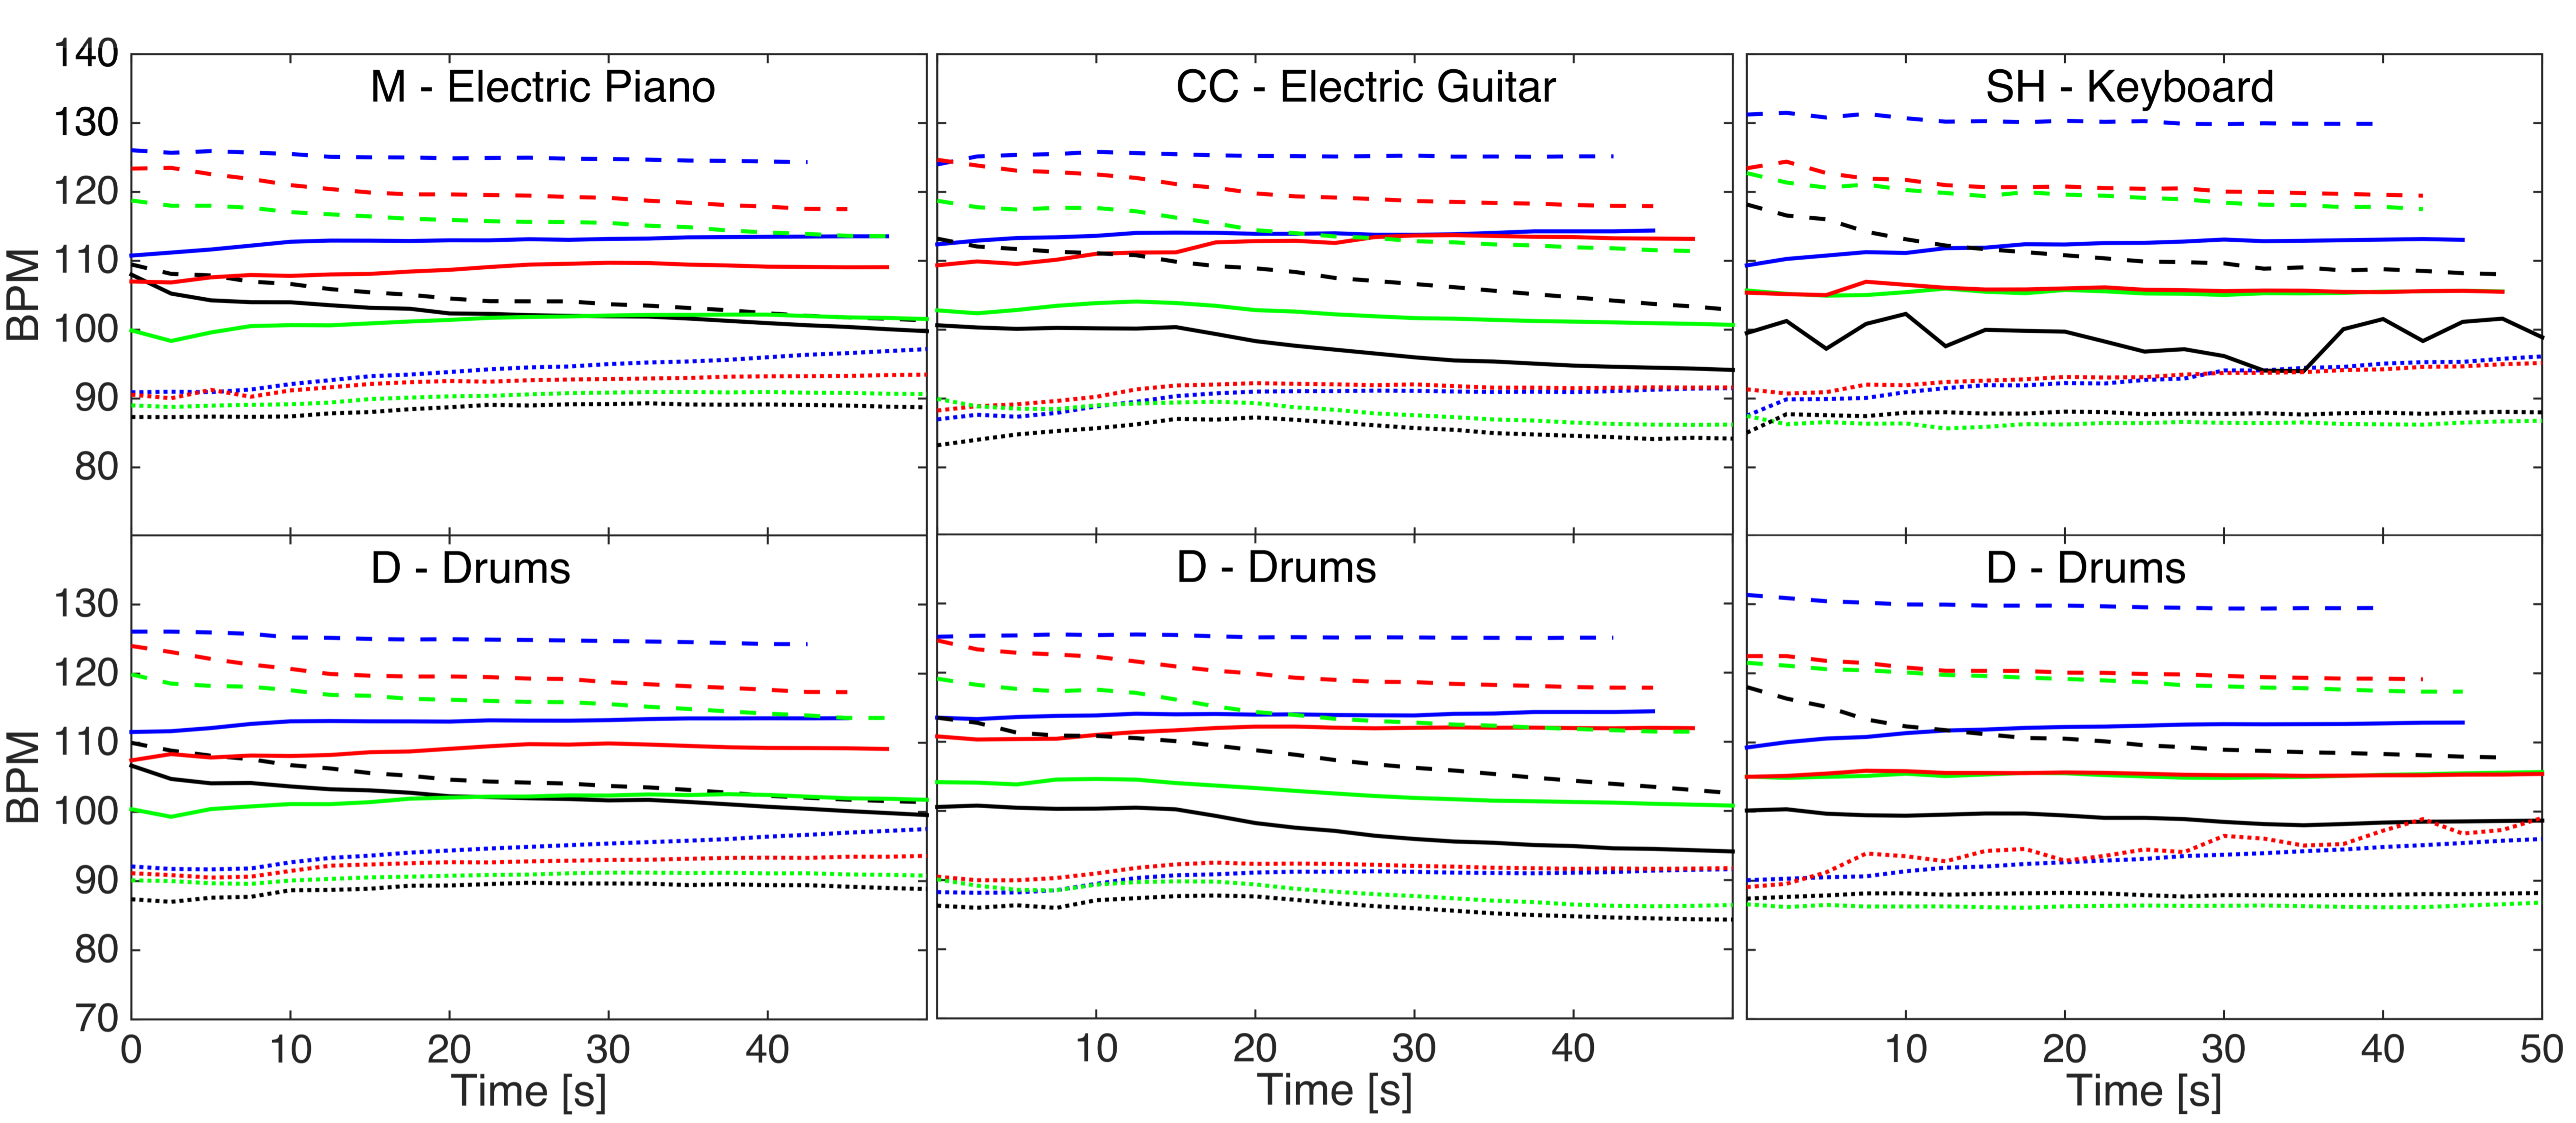
\includegraphics[width=\textwidth]{img/NMP/fig2_wider}
  \caption{BPM trend over time when playing \textit{Yellow Submarine} with Drums, combined with different parts and instruments, for various values of end-to-end delays $T_{tot}$ (identified by the color) and reference BPM $\delta$, identified by the type of line (solid, dashed, dotted).}
 \label{fig:NMP:drums} 
\end{figure}


%
%\begin{figure}[!tb]
%  \centering
%  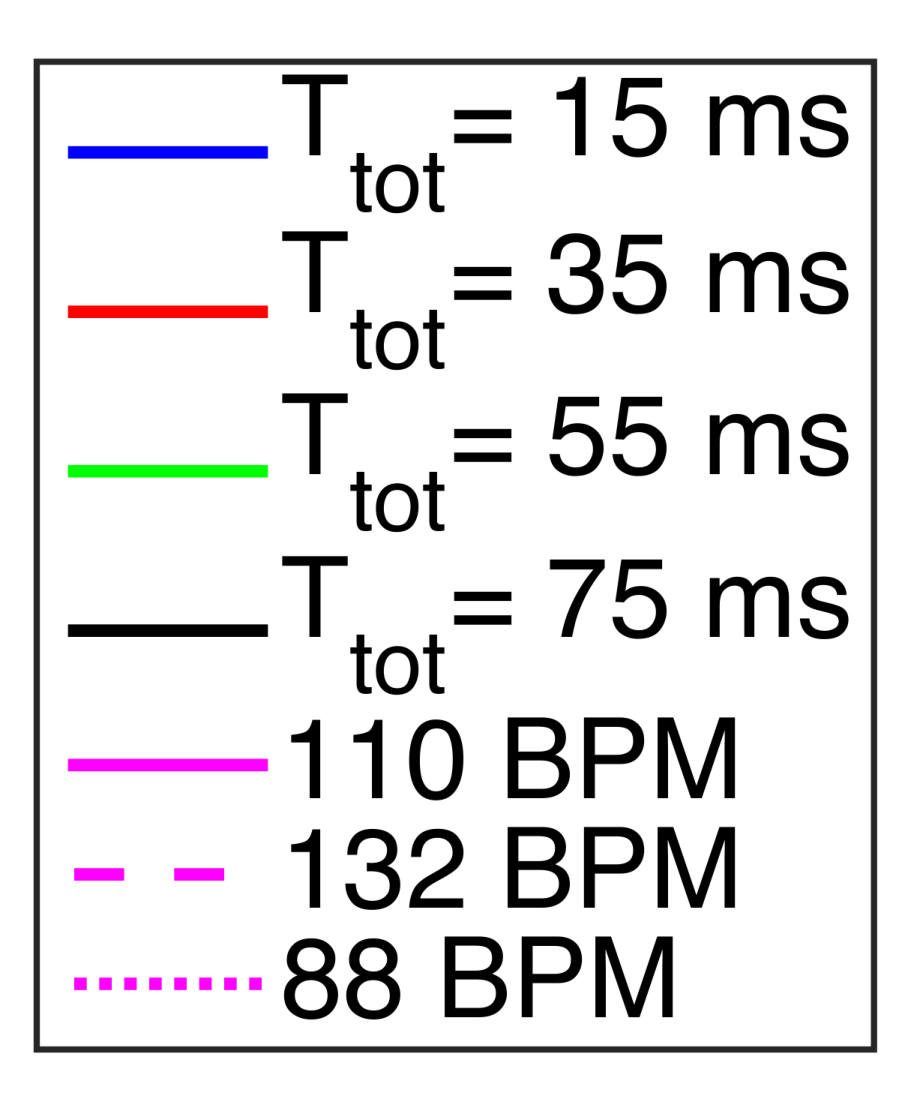
\includegraphics[width=0.2\textwidth]{img/NMP/legend_smaller}
%  \caption{Legend for Figures \ref{fig:NMP:melody} and \ref{fig:NMP:drums} }
% \label{fig:NMP:legend} 
%\end{figure}


When two homo-rhyrthmic parts (those that are expected to keep a steady tempo, such as CC and SH) are combined, $b(t_n)$ tends to remain almost constant (see Figure \ref{fig:NMP:melody}, on the right-hand side, where a slight negative slope occurs only at $\delta=132$ BPM).
A similar behavior is observed when M, CC or SH combine with Drums (See Figure \ref{fig:NMP:drums}), despite the fact that the two parts are not always homo-rhythmic. This is due to the fact that drums tend to have a very specific rhythmic ``leading role" in western music, therefore the other musicians generally tend to follow the drummer.

Based on the above results, we conclude that the choice of the combination of instruments and parts has a significant impact on the capability of the musicians to keep a steady tempo. 
In the next Section, we will give a more in-depth analysis of the impact of single rhythmic and timbral features characterizing the specific combination of parts and instruments on the subjective and objective performance quality metrics.

\subsection{Quantitative evaluation}
We now analyze the impact of different end-to-end delays $T_{tot}$ on the subjective quality metric $D_{perc}$ and on the BPM slope $\kappa$, for various values of the rythmic and timbral features described in Section \ref{sec:NMP:domain}. The interaction quality rating $Q_{perc}$ resulted to be strongly correlated to $D_{perc}$, therefore for the sake of brevity we do not report such results.


%\subsubsection{Dependency of Quality Metrics on Rythmic Features}
\begin{figure}[!tb]
\begin{flushright}
  \subfloat[Subjective Perception of Delay $D_{perc}$]{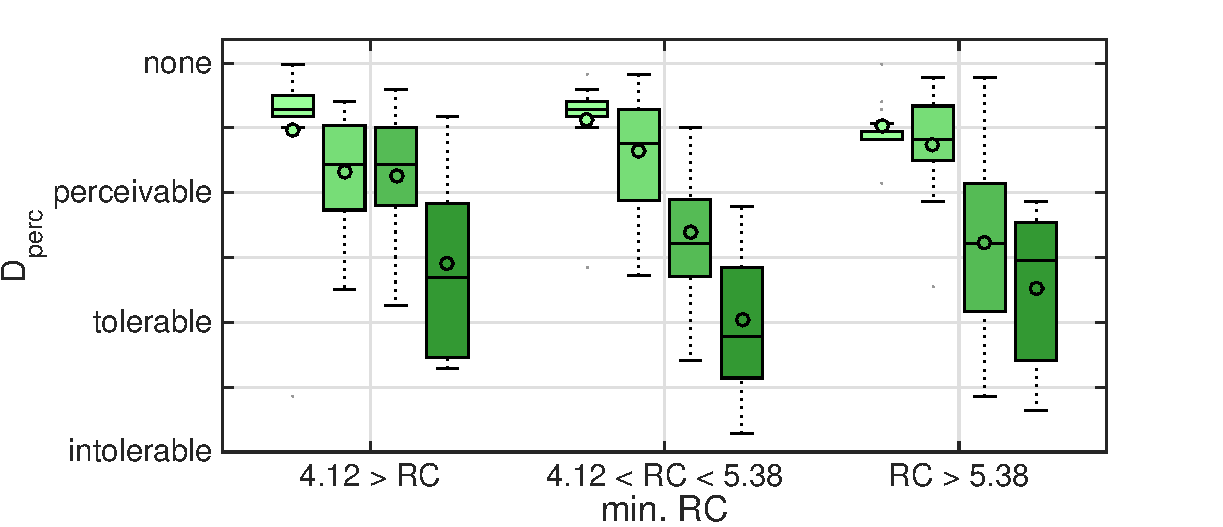
\includegraphics[width=.77\textwidth]{img/NMP/minRC_PD}\label{fig:NMP:minRC_SubjPerc}}  \hfil
  \subfloat[Average BPM Linear Slope $\kappa$]{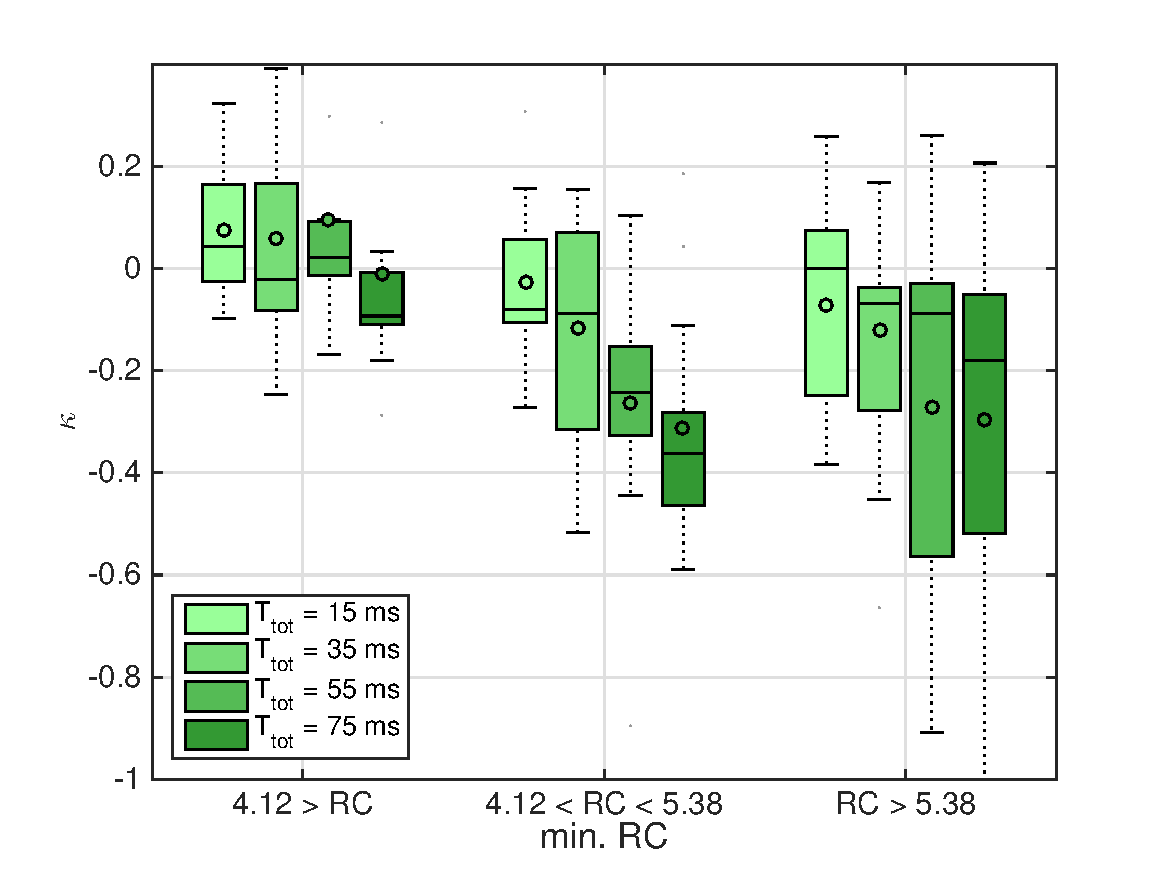
\includegraphics[width=.72\textwidth]{img/NMP/minRC_BPM}\label{fig:NMP:minRC_LinSlope}}        
\end{flushright}
\caption{Dependence of $\kappa$ and $D_{perc}$ on the minimum Rythmic Complexity $RC$ for different values of $T_{tot}$.}
\label{fig:NMP:minRC}
\end{figure}


 

For every recording, we consider the maximum and minimum values of each feature among the two parts and instruments played by the musicians. For example, in test session 2 (see Table \ref{tab:NMP:sessions}) when performing \textit{Bolero}, the minimum event density ($ED$) is 2.01 ($ED$ of the D part) and the maximum $ED$ is 2.14 ($ED$ of the M part). Conversely, the minimum rhythmic complexity ($RC$) is 5.53 (on the M part) and the maximum $RC$ is 6.03 (on the D part).

\begin{figure}[!tb]
\begin{flushright}
  \subfloat[Subjective Perception of Delay $D_{perc}$]{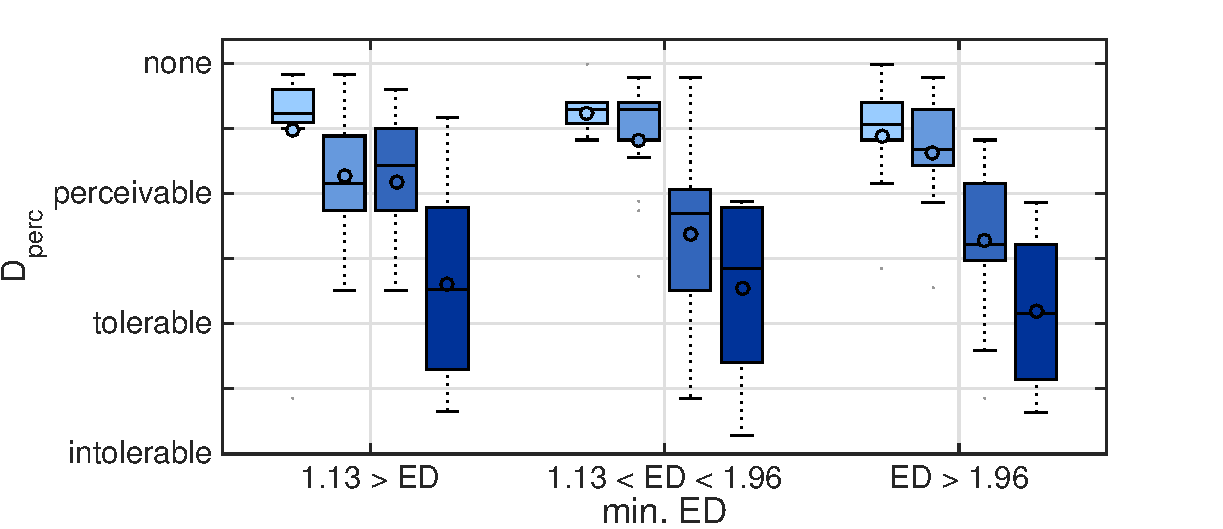
\includegraphics[width=.77\textwidth]{img/NMP/minED_PD}\label{fig:NMP:minED_SubjPerc}}  \hfil
  \subfloat[Average BPM Linear Slope $\kappa$]{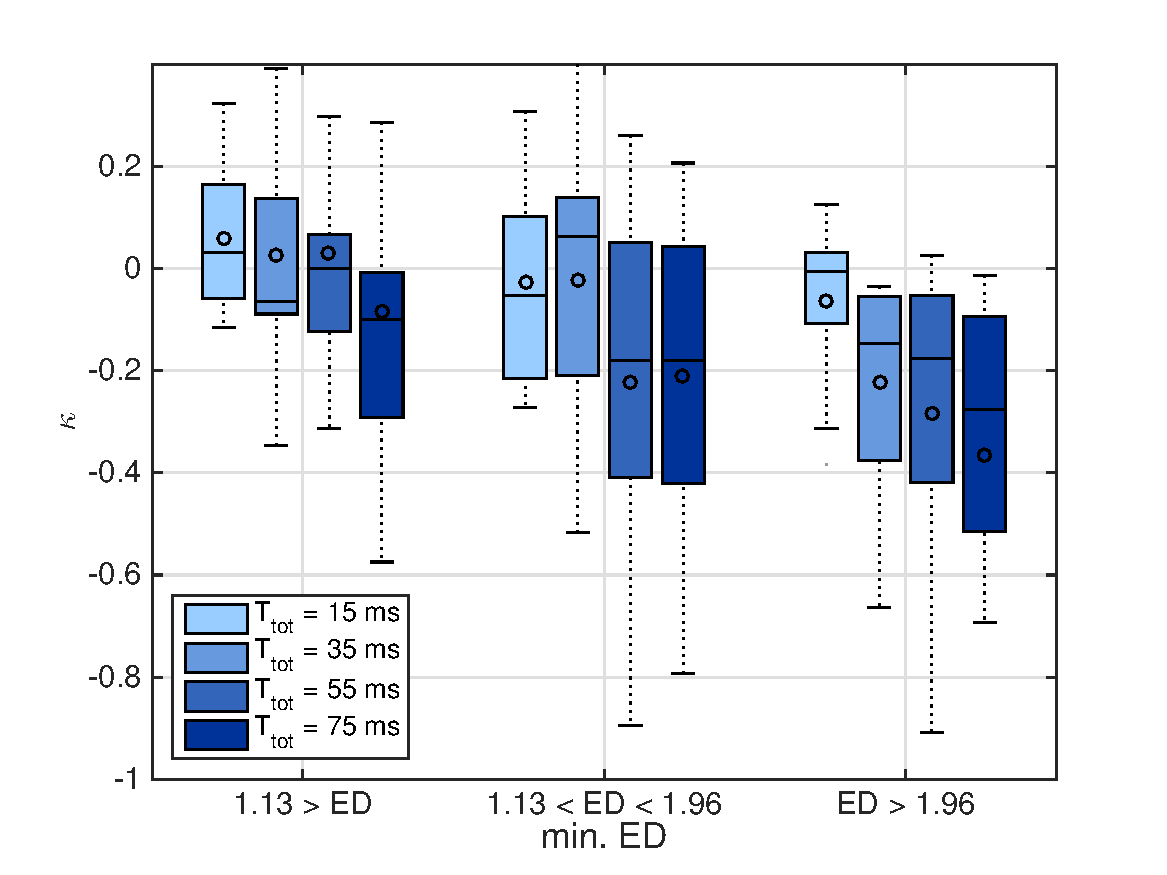
\includegraphics[width=.72\textwidth]{img/NMP/minED_BPM}\label{fig:NMP:minED_LinSlope}}        
\end{flushright}
\caption{Dependence of $\kappa$ and $D_{perc}$ on the minimum Event Density $ED$ for different values of $T_{tot}$}
\label{fig:NMP:minED}
\end{figure}

Figure \ref{fig:NMP:minRC_SubjPerc} reports the subjective delay perception $D_{perc}$ attributed by the pairs of testers to their performances, for different values of $T_{tot}$, as a function of the minimum $RC$ between the two parts. For the sake of clarity, only four values of $T_{tot}$ are reported, where $T_{tot}=T_{proc}=15$ ms is considered as benchmark. 

\begin{figure}[!tb]
\begin{flushright}
  \subfloat[Subjective Perception of Delay $D_{perc}$]{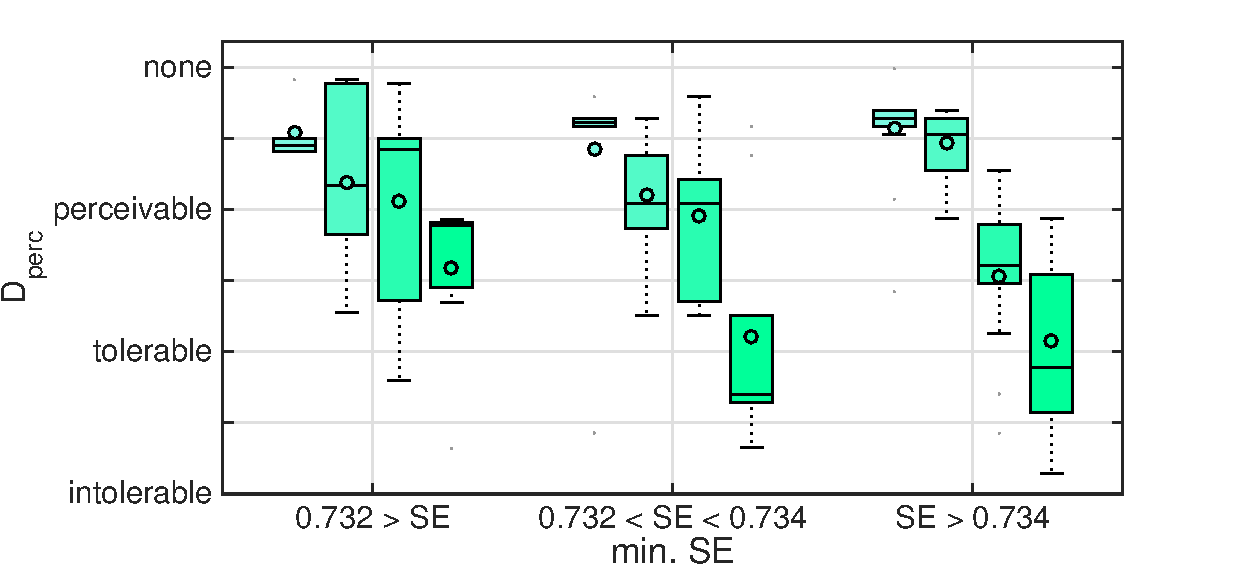
\includegraphics[width=.77\textwidth]{img/NMP/minSE_PD}\label{fig:NMP:minSE_SubjPerc}}  \hfil
  \subfloat[Average BPM Linear Slope $\kappa$]{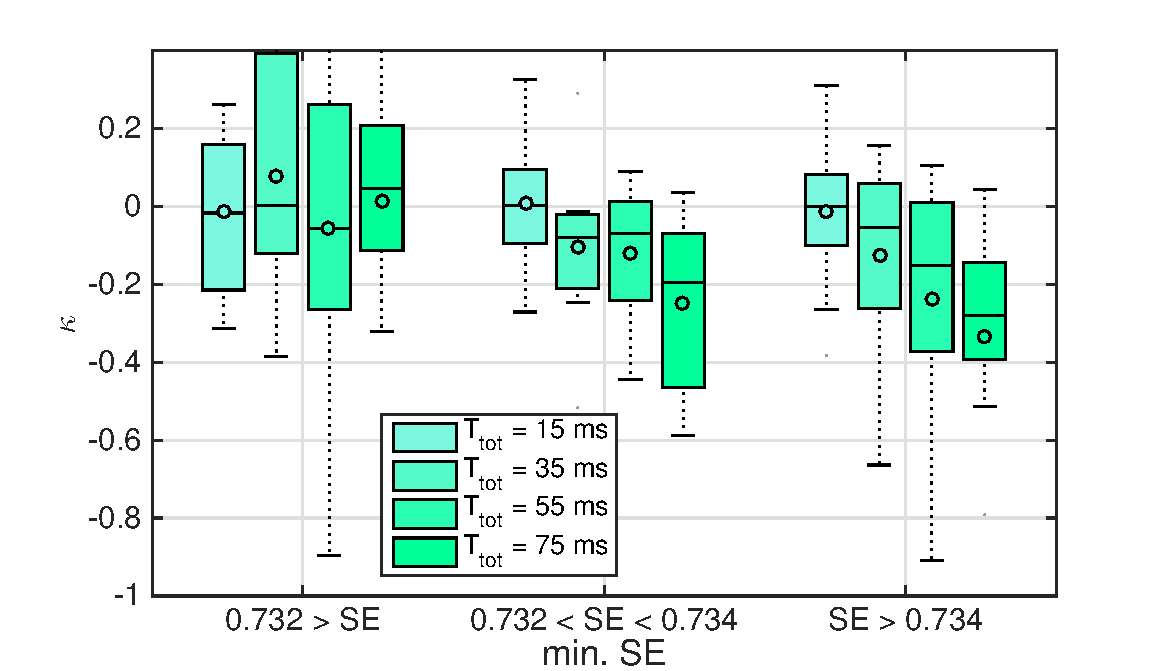
\includegraphics[width=.72\textwidth]{img/NMP/minSE_BPM}\label{fig:NMP:minSE_LinSlope}}        
\end{flushright}
\caption{Dependence of $\kappa$ and $D_{perc}$ on the minimum Spectral Entropy $SE$ for different values of $T_{tot}$}
\label{fig:NMP:minSE}
\end{figure}


Results shows that, for a given value of minimum $RC$, the average $D_{perc}$ decreases when $T_{tot}$ increases. Moreover, for a given $T_{tot}$, increasing $RC$ also has a negative impact on the average quality rating. However, the reduction of $D_{perc}$ is more relevant for large values of $T_{tot}$. 
%Similar results are obtained when considering the subjective delay perception $D_{perc}$, averaged over the pair of performers (see Figure \ref{}).

\begin{figure}[!tb]
\begin{flushright}
  \subfloat[Subjective Perception of Delay $D_{perc}$]{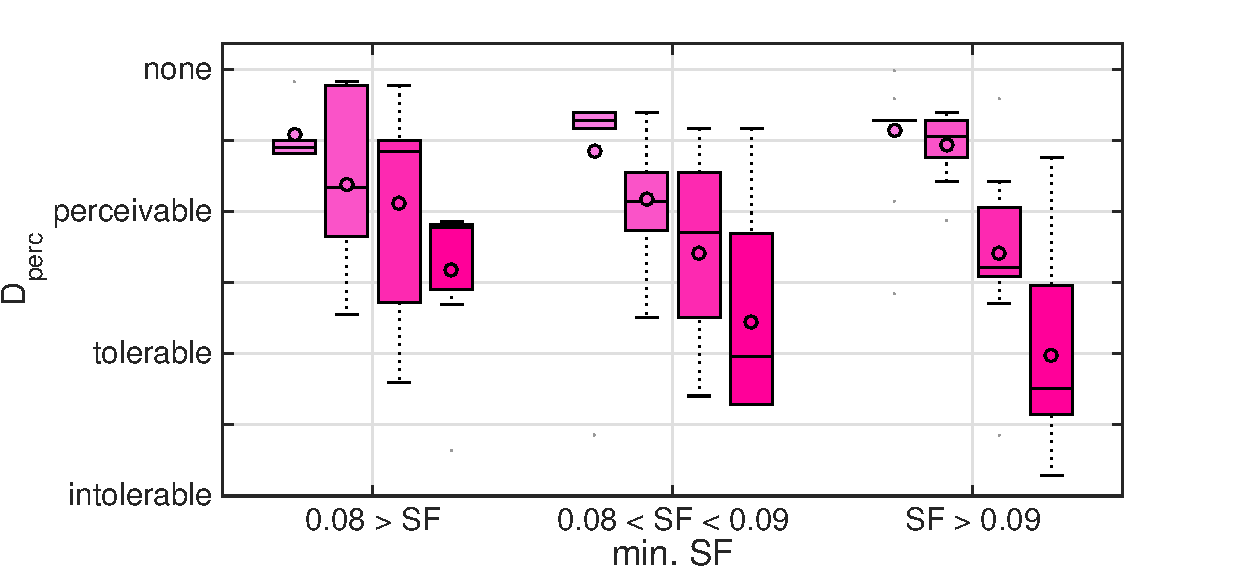
\includegraphics[width=.77\textwidth]{img/NMP/minSF_PD}\label{fig:NMP:minSF_SubjPerc}}  \hfil
  \subfloat[Average BPM Linear Slope $\kappa$]{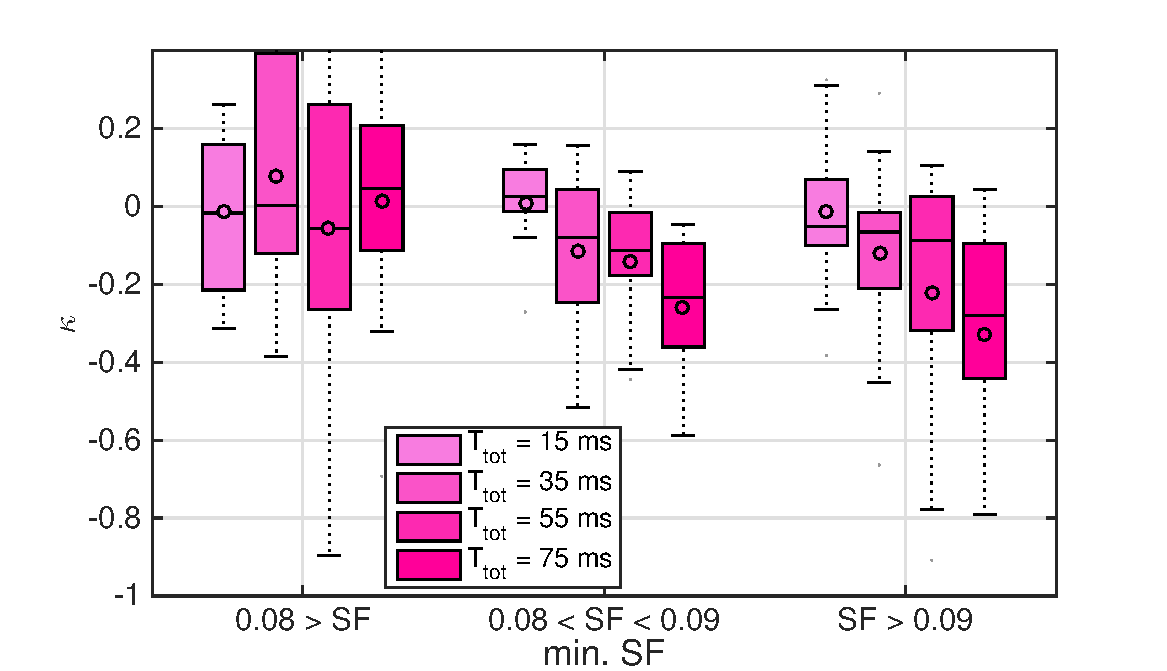
\includegraphics[width=.72\textwidth]{img/NMP/minSF_BPM}\label{fig:NMP:minSF_LinSlope}}        
\end{flushright}
\caption{Dependence of $\kappa$ and $D_{perc}$ on the minimum Spectral Flatness $SF$ for different values of $T_{tot}$}
\label{fig:NMP:minSF}
\end{figure}

We now analyze how the average BPM linear slope $\kappa$ is affected by the minimum rhythmic complexity $RC$. For large values of $RC$ (see Figure \ref{fig:NMP:minRC_LinSlope}), we found slightly negative values of $\kappa$ (which denote a tendency to slow down) even in the benchmark scenario. As expected, the need of synchronism increases when musicians are playing more complex parts and the lack of typical synchronization cues, such as eye-contact, affects the performance even in absence of network delay. However, negative slopes tend to become much steeper for large values of $T_{tot}$, which suggests that the tolerance to the delay decreases for more complex musical pieces.

\begin{figure}[!tb]
\begin{flushright}
  \subfloat[Subjective Perception of Delay $D_{perc}$]{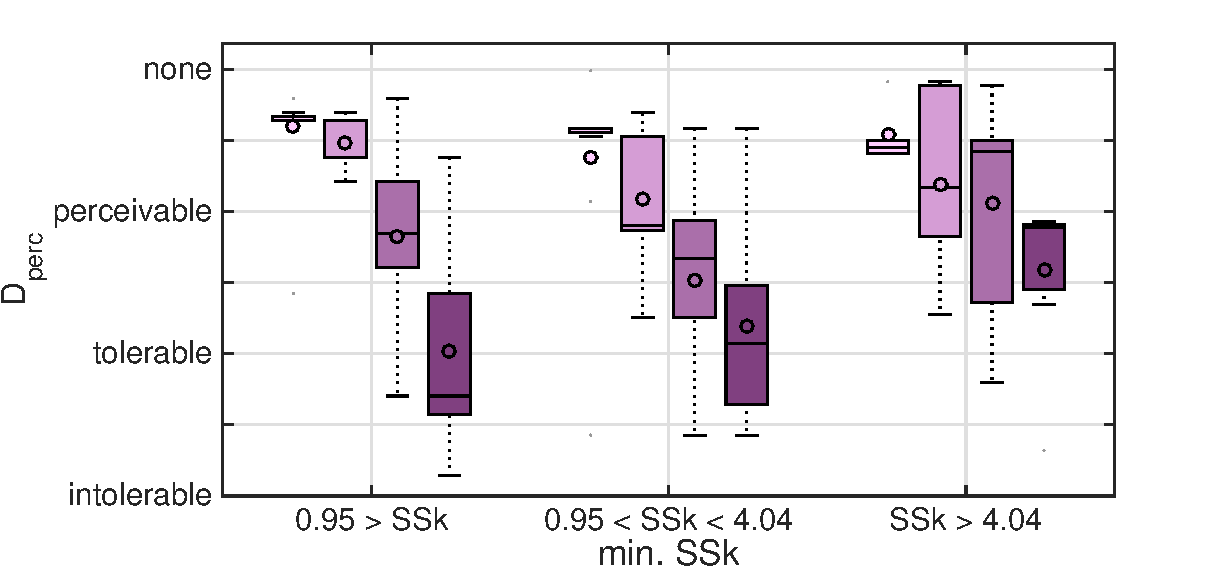
\includegraphics[width=.77\textwidth]{img/NMP/minSSk_PD}\label{fig:NMP:minSSk_SubjPerc}}  \hfil
  \subfloat[Average BPM Linear Slope $\kappa$]{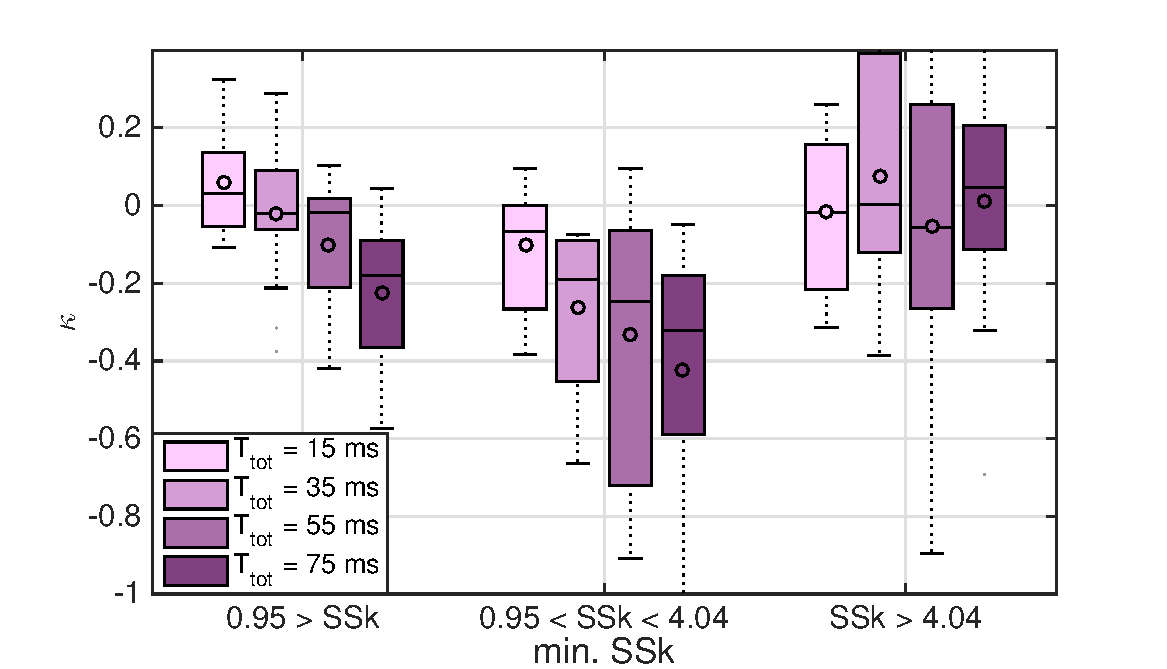
\includegraphics[width=.72\textwidth]{img/NMP/minSSk_BPM}\label{fig:NMP:minSSk_LinSlope}}        
\end{flushright}
\caption{Dependence of $\kappa$ and $D_{perc}$ on the minimum Spectral Skewness $SSk$ for different values of $T_{tot}$.}
\label{fig:NMP:minSSk}
\end{figure}

Similar conclusions can be drawn on the dependence of the perceived delay $D_{perc}$ and the objective metrics $\kappa$ on the minimum $ED$, as depicted in Figure \ref{fig:NMP:minED}, due to the non-negligible correlation that exists between $RC$ and $ED$. 
These conclusions remain substantially unvaried if, instead of considering the minimum values of $RC$ and $ED$, we consider the maxima.
%\subsubsection{Dependency of Quality Metrics on Timbral Features}

\begin{figure}[!tb]
\begin{flushright}
  \subfloat[Subjective Perception of Delay $D_{perc}$]{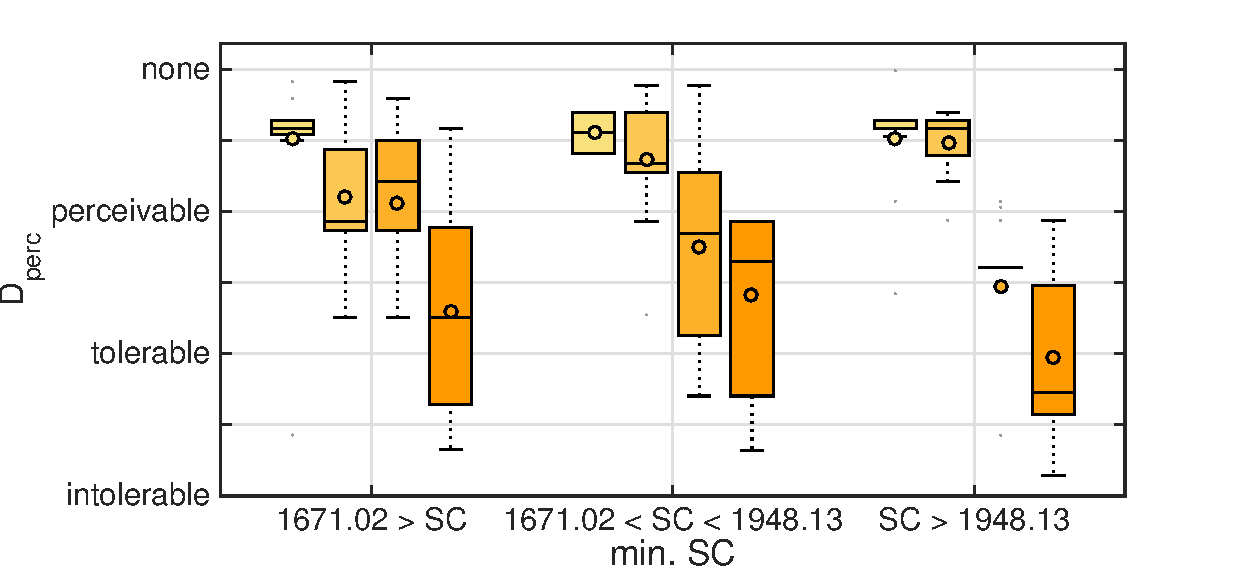
\includegraphics[width=.77\textwidth]{img/NMP/minSC_PD}\label{fig:NMP:minSC_SubjPerc}}  \hfil
  \subfloat[Average BPM Linear Slope $\kappa$]{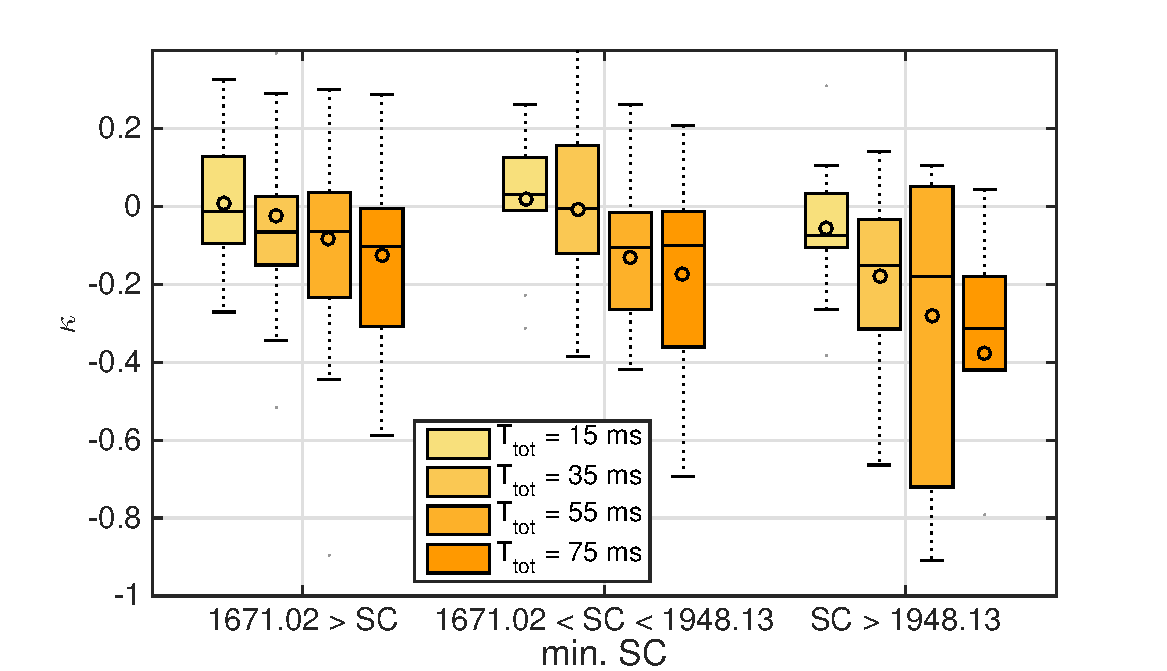
\includegraphics[width=.72\textwidth]{img/NMP/minSC_BPM}\label{fig:NMP:minSC_LinSlope}}        
\end{flushright}
\caption{Dependence of $\kappa$ and $D_{perc}$ on the minimum Spectral Centroid $SC$ for different values of $T_{tot}$.}
\label{fig:NMP:minSC}
\end{figure}



As far as timbral features are concerned, we observe that the noisiness of the instrument, which is captured by Spectral Entropy, Flatness and Spread, has a relevant impact on the perceived delay $D_{perc}$. For example, in Figures \ref{fig:NMP:minSE} and \ref{fig:NMP:minSF} we show $D_{perc}$ and $\kappa$ are affected by Spectral Entropy ($SE$) and Spectral Flatness ($SF$). We consider the minimum Entropy and minimum Flatness between the two involved instruments. Focusing on the objective metric $\kappa$ (see Figures \ref{fig:NMP:minSE_LinSlope} and \ref{fig:NMP:minSF_LinSlope}), we notice that as the $SE$ and the $SF$ increase, the tempo slowdown becomes more relevant. This impact is negligible for low network delays, but it grows significantly for fairly large values of $T_{tot}$. Similar considerations are valid for $D_perc$, as reported in Figure \ref{fig:NMP:minSE_SubjPerc}. Analogous findings also apply to the dependency of the quality metrics on the Spectral Spread (these results are not shown here for reasons of space). 

Conversely, when considering the impact of Spectral Skewness ($SSk$) and Spectral Kurtosis ($SK$) on the performance metrics, we notice that, for a given delay $T_{tot}$, a change in their values does not cause the quality to perceivably worsen (see Figure \ref{fig:NMP:minSSk}, results on $SK$ not reported for conciseness). 

Finally, when looking at the influence of the Spectral Centroid $SC$ (i.e., of sound brightness) on the subjective quality metrics, results reported in Figure \ref{fig:NMP:minSC_SubjPerc} show that the perceptual metric $D_{perc}$ does not exhibit significant fluctuations due to a varying $SC$. However, for large values of $SC$, a slight tendency to decelerate emerges in Figure \ref{fig:NMP:minSC_LinSlope}, which shows the impact of $SC$ on the objective quality metric $\kappa$.

It is also worth noticing that $D_{perc}$ is not necessarily an indicator of quality degradation of the performance, but only on the musicians' subjective perception of the end-to-end delay. However, results reported in Figures \ref{fig:NMP:minRC_SubjPerc}, \ref{fig:NMP:minED_SubjPerc}, \ref{fig:NMP:minSE_SubjPerc}, \ref{fig:NMP:minSF_SubjPerc}, \ref{fig:NMP:minSSk_SubjPerc}, \ref{fig:NMP:minSC_SubjPerc}, show that such perception is strongly affected by the timbral and rhythmic characteristics of the combination of instruments and parts. For example, in Figure \ref{fig:NMP:minSSk_SubjPerc}, the perceived network delay $D_{perc}$ is larger for high values of $SSk$ and $T_{tot}$ than the value we would have in the case of low delays. This leads us to think that the musicians' capability of estimating the network delay is biased by the perceived interaction quality of the performance.
This means that large network delays (i.e., $T_{tot}\geq 75ms$) do not prevent networked musical interaction, but they limit the selection of the instrument/part combinations. Thus, the resulting experience can be satisfactory if the performer is willing to trade flexibility and perceived interaction quality with the convenience of playing over the network.

\section{Final considerations}\label{sec:NMP:conclusions}
The NMP is a promising application to allow musicians to jam and compose songs from different physical location through the network. The network connections introduce a delay that musicians must take into account. While several network architectures can be proposed in order to reduce such delay, it is important to understand which factors affect the musicians' tolerance to it and which conditions make it easy for musicians to remotely perform.

In this Chapter, we propose an extensive evaluation of the quality of Networked Music Performances (NMPs) as a function of numerous parameters, some concerning telecommunication network delays and conditions, others involving rhythmic and timbral descriptors of the musical instruments involved. The analysis also considers the influence of the role of the instrument on such quality metrics.

In order to conduct this analysis, we implemented a testbed for psycho-acoustic tests, which emulates the behavior of a real telecommunication network in terms of variable transmission delay and jitter. %, and we quantitatively evaluated the impact of the various performance parameters on the trend of the tempo that the musicians were able to keep during the performance, as well as on the perceived quality of the musical interaction.
We model the analysis of factors that affect NMP as a linking function between the low-level and mid-level interpretation of the signal domain and the semantics expressed by the perceived and objective quality of the performance. The former allows us to objectively analyze the role of rhythmic complexity in the parts, as well as the timbral properties of the instruments that are played. The latter provides both a subjective and an objective evaluation of the performance. We use a manual analysis of the correlation between the two domains to understand which factors of the music performance are involved.

We found that the possibility of enjoying an interactive networked musical performance is not only a function of the total network delay, but it also depends on the role and the timbral characteristics of the involved musical instruments, as well as the rhythmic complexity of the performance. When playing more rhythmically complex pieces, musicians exhibit a more pronounced tendency to decelerate for higher network latencies. Nonetheless, the rhythmical complexity does not significantly worsen their perception of the delay and of the interaction quality.
Among the timbral features, instruments with a higher Spectral Entropy and Spectral Flatness (such as guitars and drums) lead to larger tempo slowdown in case of higher network delays. In addition, they also amplify the negative impact of network delay on the perceived delay and interaction quality.

With this results in mind, we are able to assess whether a certain NMP can be successful given the network delay and the combination of parts and instruments that are performing remotely.
%This paper investigates the tolerance of remotely interacting musicians towards adverse network conditions. We do so for various musical instruments and music genres, as a function of rhythmic complexity and tempo. 

 



%
%\section{Acknowledgments}
%The authors are grateful to Prof. Alexander Car\^{o}t for his generous assistance with the SoundJack software, and to all the people that were involved in the psycho-perceptual tests, particularly Antonio Canclini, Bruno Di Giorgi, Lorenzo Dainelli, Niccol\'{o} Dainelli, Davide Pradolini and Simone Pradolini.
